\subsection{Booster neutrino beam, BNB}

A Booster Neutrino Beam fires neutrinos directly into the time projection chamber of an experiment at such speeds that the particles can always be assumed to be forward-going. This technicality allows for a reasonably straightforward removal of backgrounds such as cosmogenic neutrinos, which would enter the time projection chamber (TPC) from all angles \cite{sbn}. 

The beam is formed by firing protons at a beryllium target which produces a hadronic beam consisting mainly of pions. The pions in this beam are then focussed and polarised in order for them to go on to decay to mostly the dominant channel $\mu ^{ + }$ and $\nu _{ \mu }$ \cite{sbn}, since the branching ratio of pions decaying to electrons over muons is on the order of $\sim 10 ^{ 4 }$ times smaller due to the relation given in equation~(\ref{eq:BR}) \cite{BR}.

\begin{equation}\label{eq:BR}
    R_{ \pi } = \left( \dfrac{ m_{ e } }{ m_{ \mu } } \right) ^{2} \left( \dfrac{ m_{ \pi }^{ 2 } - m_{ e } ^{ 2 } }{ m_{ \pi } ^{ 2 } - m_{ \mu } ^{ 2 } } \right) ^{ 2 } \sim 10^{-4}
\end{equation}

    
\subsection{Liquid argon time projection chambers, LArTPC}     
    
    In current and future neutrino experiments such as DUNE and the short baseline neutrino (SBN) program (SBND, MicroBooNE and ICARUS), liquid argon is the target material of the detector. Argon in this form is used due to its stability and purity as a noble gas, its high denisty and its low cost. These properties lead to resolution capabilities on the order of the Bubble Chamber experiments, which allows for high certainty in distinguishing between interactions and ultimately optimises the resolving power of the experiment \cite{larRes}.


    %LArTPC
    \begin{figure}[h!]
        \center
        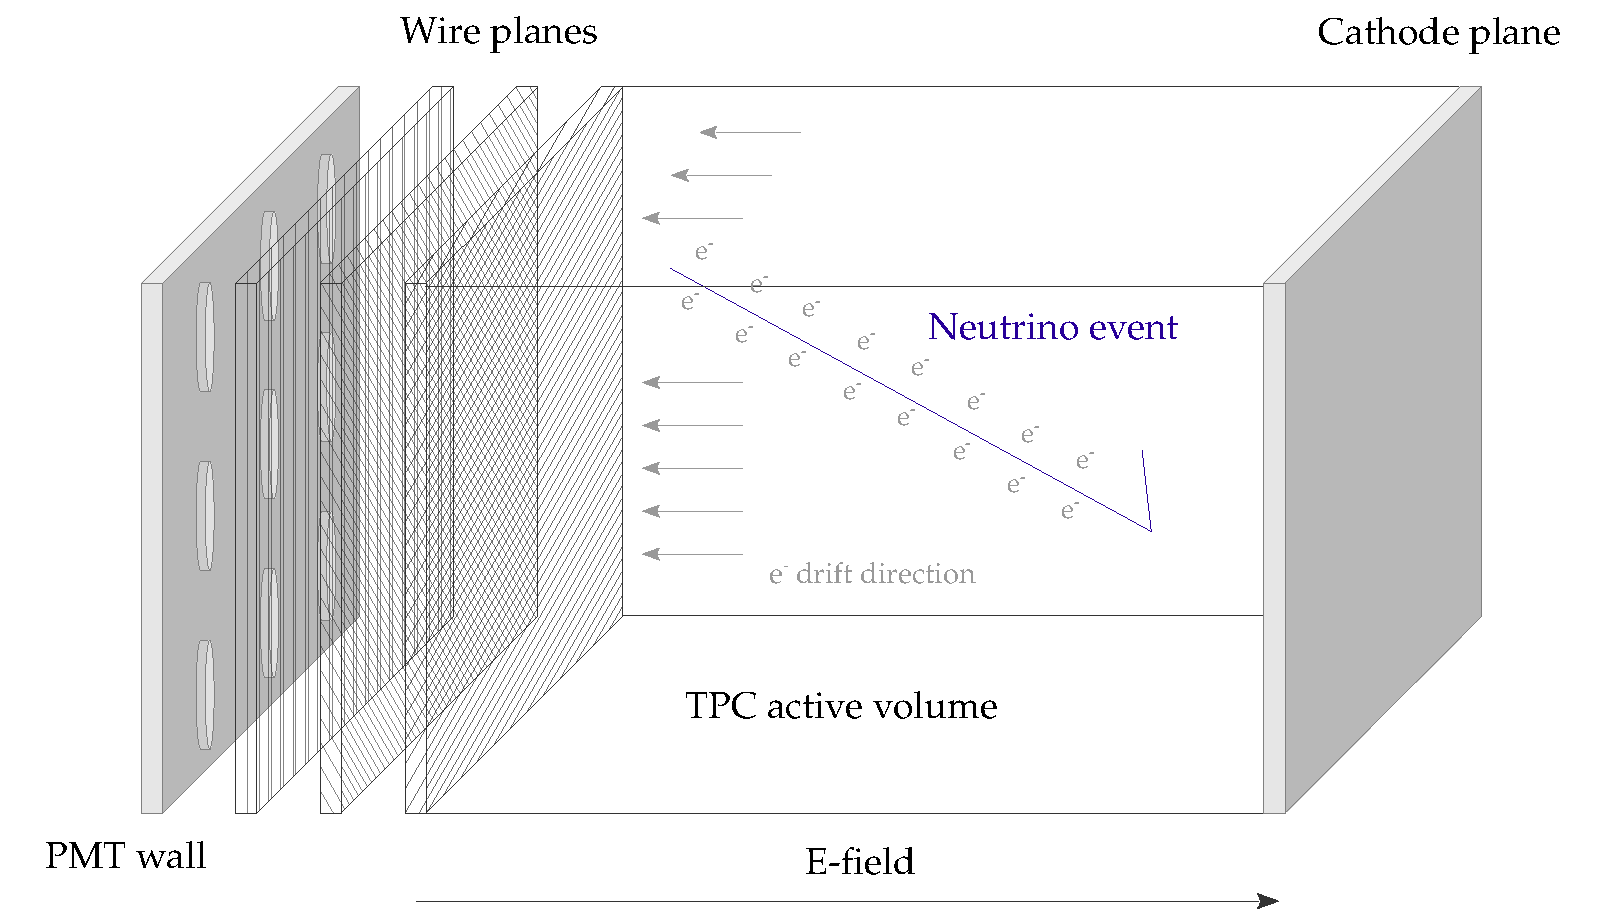
\includegraphics[width=\textwidth]{images/LArTPC.pdf}
        \caption{LArTPC}
        \label{fig:lartpc}
    \end{figure}

        

    % Plan
    \begin{itemize}

        \item LArTPC general functionality
        \item LArTPC resolution benefits
        Bubb-chamb


        \item Comparison with other detector materials
    
    \end{itemize}

    An example event display on liquid argon is shown in Figure~\ref{fig:ev_disp} \cite{evDisp}
    % Event display
    \begin{figure}[h!]
        \center
        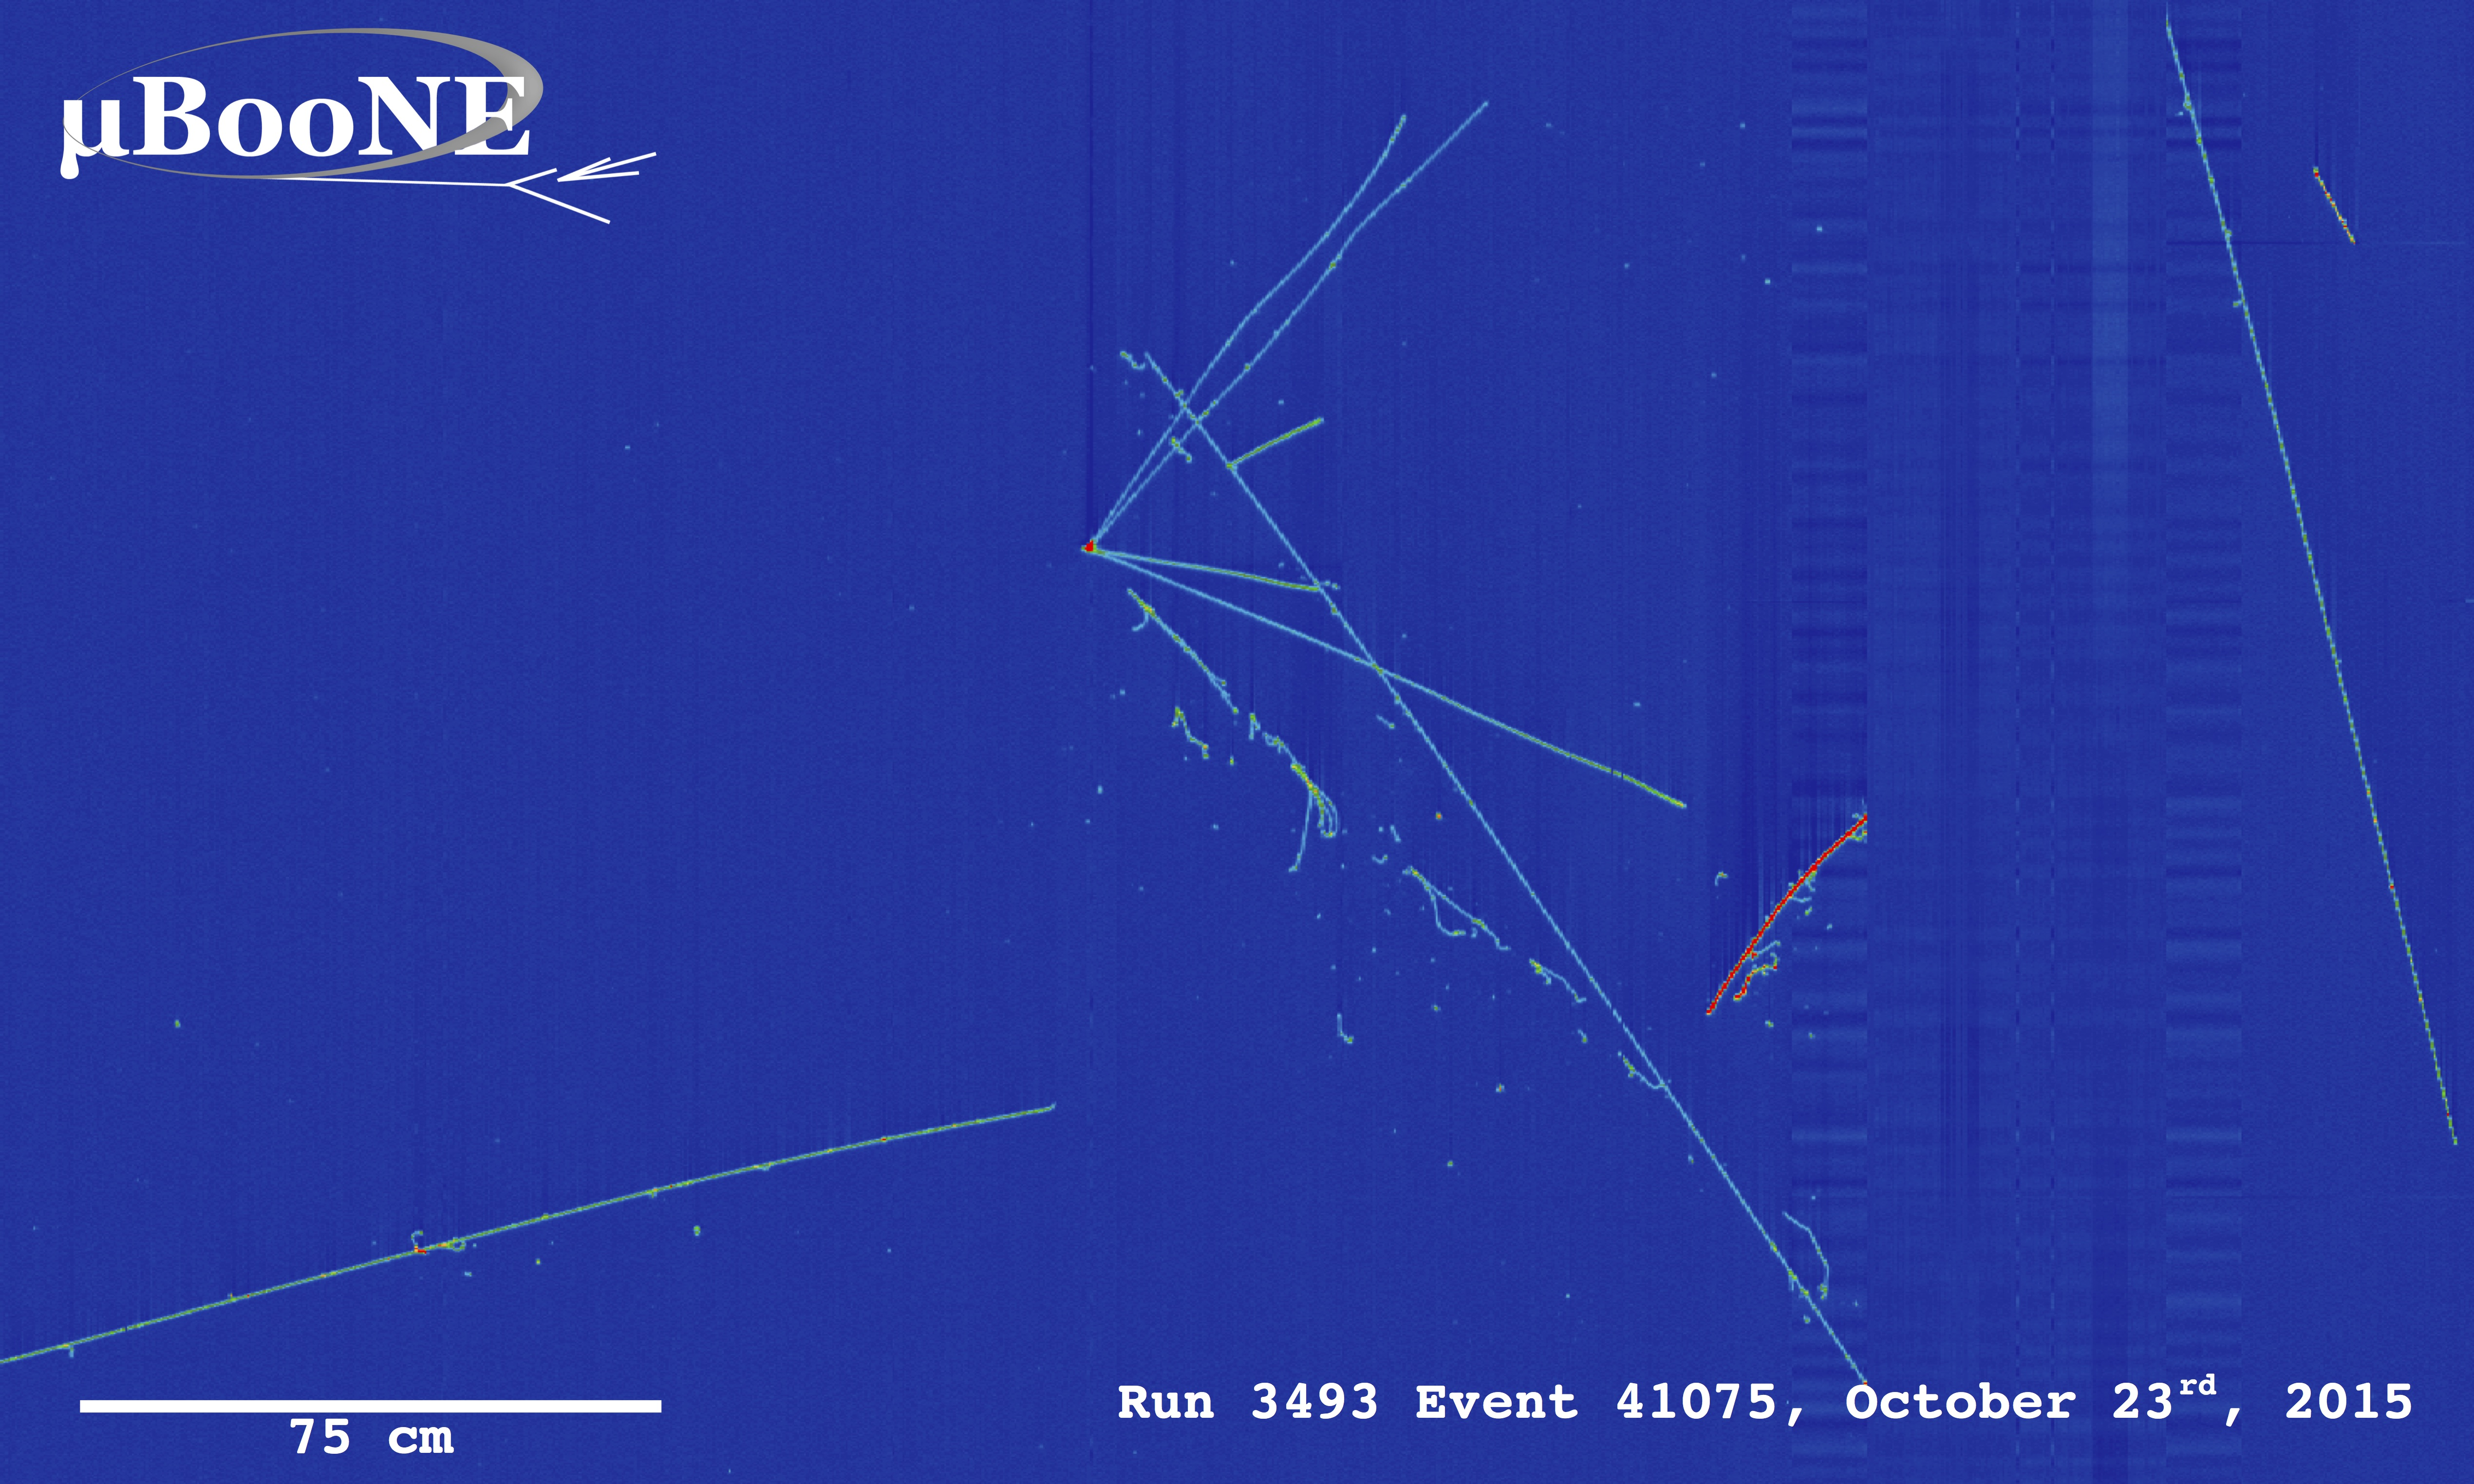
\includegraphics[width=.8\textwidth]{images/uboone_ev.png}
        \caption{MicroBooNE}
        \label{fig:ev_disp}
    \end{figure}


\subsection{SBND}    

    % Plan
    \begin{itemize}
    
        \item SBND specifics

        \begin{itemize}

            \item Dimensions
            \item Beamline
            \item Flux
            \item Statistics
            \item Physics goals

        \end{itemize}
        
        \item Cross-section precision capabilites

    \end{itemize}

    % Table
    \renewcommand{\arraystretch}{1.3}
\begin{center}
\begin{tabular}{lll}
    \textbf{Process} & & \textbf{No. Events} \\ 
    \hline\hline
    \multicolumn{3}{c}{\textit{\( \nu_{ \mu } \) Events }}\\
        CC 0 \( \pi \)                 & \( \nu_{ \mu } N \rightarrow \mu + Np \)                            & \textbf{3,551,830} \\
        CC 1 \( \pi^{ \pm } \)         & \( \nu_{ \mu } N \rightarrow \mu + nucleons +  1\pi^{ \pm } \)      & \textbf{1,161,610} \\
        CC \( \geq 2\pi^{ \pm } \)     & \( \nu_{ \mu } N \rightarrow \mu + nucleons + \geq 2\pi^{ \pm } \)  & 97,929 \\
        CC \( \geq 1\pi^{ 0 } \)       & \( \nu_{ \mu } N \rightarrow \mu + nucleons + \geq 1\pi^{ 0 } \)    & 497,963 \\
        \hline        
        NC 0 \( \pi \)                 & \( \nu_{ \mu } N \rightarrow nucleons \)                            & 1,371,070 \\
        NC 1 \( \pi^{ \pm } \)         & \( \nu_{ \mu } N \rightarrow nucleons +  1\pi^{ \pm } \)            & 260,924 \\
        NC \( \geq 2\pi^{ \pm } \)     & \( \nu_{ \mu } N \rightarrow nucleons + \geq 2\pi^{ \pm } \)        & 31,940 \\
        NC \( \geq 1\pi^{ 0 } \)       & \( \nu_{ \mu } N \rightarrow nucleons + \geq 1\pi^{ 0 } \)          & 358,443 \\
        \hline\hline
        \multicolumn{2}{l} {Total \( \nu_{ \mu } \) \& \( \nu_{ e } \) events }                              & \textbf{7,251,948} \\
\end{tabular}
\end{center}

    
 \clearpage
